can %% CyclicEnv --- Environmental Modelling & Software (Elsevier)
%% Overleaf: set main document to main.tex; compiler = pdfLaTeX
\documentclass[preprint,12pt,authoryear,review]{elsarticle}

\usepackage[T1]{fontenc}
\usepackage[utf8]{inputenc}
\usepackage{amsmath,amssymb}
\usepackage{booktabs}
\usepackage{graphicx}
\usepackage{hyperref}
\usepackage{listings}
\usepackage{xcolor}
\usepackage{doi}
\usepackage{url}
\usepackage{tabularx}
\usepackage{multirow}

\journal{Environmental Modelling \& Software}

\lstset{
  basicstyle=\ttfamily\footnotesize,
  breaklines=true,
  frame=single,
  columns=fullflexible,
  keepspaces=true,
  language=Python
}

\hypersetup{colorlinks=true,linkcolor=blue,citecolor=blue,urlcolor=blue}
\graphicspath{{figures/}}

\begin{document}

\begin{frontmatter}

\title{CyclicEnv: an open Gymnasium environment and benchmark for learning unobserved water fate in a cyclic-irrigation paddy district}

\author[aff1]{Author One\corref{cor1}}
\ead{author.one@example.edu}
\author[aff1]{Author Two}
\address[aff1]{Affiliation to be completed}
\cortext[cor1]{Corresponding author}

\begin{abstract}
Cyclic irrigation reuses paddy drainage by pumping it back into the supply canal, but the subsurface part of that reuse---lateral seepage through bunds and its recapture at the pumping station---is not measured at plot scale and is known only as a district water-balance residual. We present CyclicEnv, an open-source Python package that turns the published two-season water balance of the Imbanuma cyclic-irrigation district \citep{okura2025} into a Gymnasium reinforcement-learning and inverse-modelling environment over 4,925 paddy polygons. Surface irrigation and drainage are supplied as known forcing, so learning concentrates on the unobserved partition of each plot's leftover water into same-day recapture, neighbour exchange and on-plot storage. Three registered learner slots---a farmer policy, a leftover-ratio model and a neighbour-head hop law---receive different observation channel packs that can be hidden or shown for ablation. An optional Copernicus Data Space client retrieves Sentinel-2 scenes over the district. Year-holdout protocols and reference results establish what a year-invariant capture field can and cannot achieve: joint training recovers each year's Table~5 recapture pin with fidelity 0.967 and 0.969, versus 0.934--0.938 for a single-year freeze. Farmer baselines range from 0.09 to 0.99 season-total fidelity; an oracle that sees observed block totals dominates irrigation scores, and a satellite-driven rule collapses from 0.80 in the wet year to 0.21 in the dry year. Fitted hop laws can beat the physics teacher on holdout, but per-paddy variants overfit. In the known-irrigation gym, a zero-discharge policy obtains the highest mean reward among the rules tested. CyclicEnv is offered as a stable, reproducible benchmark for district-scale water-fate learning and simulation-based optimisation, not as a claim of a best algorithm.
\end{abstract}

\begin{highlights}
\item Open Gymnasium environment for a 4,925-paddy cyclic-irrigation district
\item Known pump and drainage forcing isolates unobserved leftover water fate
\item Separate farmer, ratio and hop-law slots with per-role observation masks
\item Joint two-year leftover capture reaches 0.97 fidelity to water-balance pins
\item Baselines expose year instability, oracle leakage and a strong zero-discharge null
\end{highlights}

\begin{keyword}
cyclic irrigation \sep paddy water balance \sep return-flow reuse \sep Gymnasium \sep reinforcement learning environment \sep inverse modelling \sep simulation optimisation \sep partial observability \sep Sentinel-2 \sep reproducible benchmark
\end{keyword}

\end{frontmatter}

%% ------------------------------------------------------------------
\section*{Software availability}
\begin{table}[htbp]
\centering
\small
\begin{tabular}{p{0.28\linewidth}p{0.62\linewidth}}
\toprule
Item & Detail \\
\midrule
Software name & CyclicEnv (\texttt{cyclic-irrigation}; import name \texttt{cyclic}), v0.2.0 \\
Developers & [to be completed] \\
Contact & [e-mail] \\
Year first available & 2026 \\
Hardware & Standard PC; about 2\,GB RAM for a full season \\
Operating system & Windows, Linux, macOS \\
Program language & Python~$\geq$\,3.10 \\
Dependencies & numpy, pandas, scipy, requests; optional gymnasium, geopandas, xarray \\
Installation & \texttt{pip install -e ".[ems]"} \\
Gymnasium IDs & \texttt{Cyclic-Imbanuma-v0}, \texttt{Cyclic-Imbanuma-Open-v0} \\
Tests & 96 unit and integration tests \\
Reproduction & \texttt{python scripts/ems\_experiments.py} \\
Licence & MIT \\
Availability & [repository URL and Zenodo DOI pending] \\
\bottomrule
\end{tabular}
\end{table}

%% ------------------------------------------------------------------
\section{Introduction}
\label{sec:intro}

\subsection{Cyclic irrigation and unobserved leftover water}

In flat, low-lying paddy districts, cyclic irrigation collects drainage in a main canal and pumps it back into the supply \citep{takeda1997,hama2010}. The practice reduces lake or river withdrawals and can retain nutrients and suspended solids inside the district. \citet{okura2025} monitored the Shiroyama--Jinbee area of the Imbanuma Land Improvement District (Chiba, Japan) in 2021 and 2022 with pump records and ADCP drainage measurements. Subsurface lateral flow from paddies emerged as a large residual term, and drought changed both water-use efficiency and the cyclic reuse ratio.

That residual is the modelling target. Plot-scale leftover $L = IR + R - D - ET$ is not observed paddy by paddy; only season block totals and pump-station recapture $LFV_{\mathrm{pump}}$ are known. Bund seepage and preferential pathways move water laterally \citep{walker1986,janssen2009}, and toposequence water-balance models make lateral movement first-class \citep{tsubo2007}. Watershed tools such as SWAT-Paddy improve ponding representation but still under-represent rapid return flow through drainage systems \citep{tsuchiya2018}. CyclicEnv does not invent a new field campaign; it turns Okura's published identities into a learnable software problem.

Accounting language matters. Irrigation ``efficiency'' gains can raise basin consumption when return flows are re-used downstream \citep{perry2007,grafton2018}. The package therefore scores reuse and capture ($LFV_{\mathrm{pump}}/LfA$) and keeps surface irrigation and drainage as known forcing rather than claiming ``saved'' water from a black-box policy.

\subsection{Learning environments and open environmental software}

Sequential decision tools need a shared contract: spaces, \texttt{reset}/\texttt{step}, rewards and seeds \citep{sutton2018}. Gymnasium provides that contract \citep{towers2024}. Agricultural gyms wrap process models for fertilisation or field irrigation \citep{overweg2021,gautron2022,kelly2021,kelly2024}. Basin tools such as MORL4Water address reservoir networks \citep{osika2026}. None of these packages represents thousands of paddies exchanging water through bunds into a shared cyclic pool, with the key flux known only as an aggregate residual.

Simulation-based control of water systems treats the simulator as fixed and searches policies on top \citep{giuliani2021}. \emph{Environmental Modelling \& Software} has a parallel line of open water-modelling software---Pywr \citep{tomlinson2020}, Pywr-DRB \citep{hamilton2024}, pytRIBS \citep{raming2025}---that sets the packaging bar CyclicEnv aims to meet. Stable-Baselines3-style learners are an intended client API \citep{raffin2021}.

\subsection{Purpose, contributions and stance}

We follow EMS guidance on credible model development: state purpose and data roles, evaluate against held-out information, use several performance measures, and publish code and workflows \citep{jakeman2006,bennett2013,hutton2016,lemmen2024}. FAIR principles for research software apply \citep{barker2022}. Year splits matter for learned hydrology \citep{gauch2021}; equifinality warns that many leftover fields can hit the same pin \citep{beven2006}. The scientific stance is hybrid process plus learning \citep{reichstein2019,nearing2021}: FAO-56 and Okura identities stay fixed; only the unobserved leftover partition and optional hop laws are learnable. Role-specific observation packs make the problem partially observable by design \citep{kaelbling1998}.

The contributions of this article are:
\begin{enumerate}
\item A pip-installable Gymnasium environment of a real cyclic-irrigation district (4,925 paddies, two seasons), with registered environment IDs and a native multi-role API.
\item A decomposition into three registered slots---farmer, leftover ratio and hop law---with known surface forcing, aggregate constraints and simulator teachers kept separate.
\item Per-role observation channel packs that support partial-observability studies and block obvious shortcuts.
\item Year-holdout evaluation protocols and reference results, including negative and degenerate findings.
\item Optional Copernicus Data Space access for Sentinel-2 over the district.
\end{enumerate}
We do not claim a new hydrological measurement, unique identification of subsurface paths, or a state-of-the-art learning algorithm.

%% ------------------------------------------------------------------
\section{Study system and data}
\label{sec:data}

\subsection{Site and season}

The environment represents the Shiroyama--Jinbee cyclic irrigation area beside Lake Kita-Imbanuma \citep{okura2025}. The district is divided into North and South blocks drained by a main drainage canal that converges at a pumping-station pool; the pool supplies irrigation to both blocks, with a lake withdrawal making up any shortfall. The irrigation season runs from 17~April to 25~August (131 days). Two seasons are available: 2021 (wet) and 2022 (dry). The parcel layer contains 4,925 paddy polygons, of which 2,061 lie inside the cyclic-irrigation command area; the rest provide spatial context and are excluded from the recapture pins.

\subsection{Forcing, constraints and teachers}

Table~\ref{tab:roles} separates every data source by its role. This separation is the central design decision: it determines what a learner may see, what it is scored against, and what cannot be claimed.

\begin{table}[htbp]
\centering
\footnotesize
\caption{Data roles in CyclicEnv.}
\label{tab:roles}
\begin{tabular}{p{0.18\linewidth}p{0.28\linewidth}p{0.28\linewidth}p{0.16\linewidth}}
\toprule
Role & Quantity & Source & Resolution \\
\midrule
Known forcing & Block irrigation $IR$, lake withdrawal $W$ & Okura Fig.~8, digitised & daily, per block \\
Known forcing / label & Block surface drainage $D$ & Okura Fig.~6 monthly ADCP, scaled by 0.881 & monthly shape \\
Aggregate constraint & $LfA$, $LFV_{\mathrm{pump}}$, storage change & Okura Tables~4--5 & season totals \\
Weather & Precipitation, $ET_0$ & Open-Meteo \citep{zippenfenig2023} & daily, district \\
Remote sensing & NDVI-derived $K_c \times ET_0$ & Sentinel-2 \citep{drusch2012} & per pass \\
Simulator teacher & Neighbour hop $\Delta L$ & Physics hop operator & daily, per paddy \\
\bottomrule
\end{tabular}
\end{table}

Two limitations are stated here rather than deferred. Daily irrigation series are digitised from a published figure, and daily drainage is a monthly ADCP shape rescaled to the season table. Digitised Fig.~8 North and South season volumes match Table~4 \emph{cyclic} $IR$ (about $9{,}798 \times 10^3$\,m$^3$ in 2021 and $10{,}209$ in 2022), not Table~5 $IR_{\mathrm{all}}$ (about $14{,}734$ and $15{,}414$). The package therefore pins Fig.~8 onto cyclic paddies and adds non-cyclic (NCB) supply so that $IR_{\mathrm{all}} = IR_{\mathrm{cyclic}} + IR_{\mathrm{ncb}}$. Neither product substitutes for the original campaign logger files, which the package can ingest when available.

\subsection{Remote sensing}

Satellite evapotranspiration targets follow the approach of deriving a crop coefficient from NDVI and multiplying by reference ET \citep{allen1998,erraki2007}. They are used as a scoring target and as an observation channel, not imposed as the simulated flux. A Copernicus Data Space client searches and downloads Sentinel-2 products over the district bounding box \citep{drusch2012}. Weather forcing is taken from the Open-Meteo archive \citep{zippenfenig2023}.

%% ------------------------------------------------------------------
\section{Model}
\label{sec:model}

\subsection{District identities}

The environment reproduces the water-balance identities of \citet{okura2025}. For block $b$ and season $y$, leftover (lateral flow) is the residual
\begin{equation}
L_b = IR_b + R - D_b - ET_b,
\label{eq:leftover}
\end{equation}
the pump-pool balance yields same-day lateral-flow recapture
\begin{equation}
LFV_{\mathrm{pump}} = IR_{\mathrm{all}} - W + O - D_N - D_S,
\label{eq:lfv}
\end{equation}
and the storage change retained in the blocks is
\begin{equation}
\Delta WB = LfA_N + LfA_S - LFV_{\mathrm{pump}},
\label{eq:dwb}
\end{equation}
where $LfA_b$ is block leftover volume, $W$ lake withdrawal and $O$ pool outflow. The district recapture ratio is
\begin{equation}
c_y = \frac{LFV_{\mathrm{pump},y}}{LfA_{N,y} + LfA_{S,y}},
\label{eq:cy}
\end{equation}
giving $c_{2021} = 0.7384$ and $c_{2022} = 0.7873$ from Tables~4--5.

\subsection{Plot water balance}

Each paddy carries a pond, a topsoil evaporable store and a root-zone store. Daily evapotranspiration uses the FAO-56 dual crop coefficient \citep{allen1998}, splitting evaporation from the pond or topsoil and transpiration from the root zone, with defaults TEW\,=\,25\,mm and TAW\,=\,100\,mm. Pond-to-soil infiltration through the plough pan is a physics rate proportional to pond depth. Plot leftover is
\begin{equation}
L_i = IR_i + R - D_i - ET_i.
\label{eq:plotL}
\end{equation}

\subsection{Leftover simplex}

Positive leftover at paddy $i$ is partitioned once:
\begin{equation}
L_i^{+} = \big(k^{\mathrm{cap}}_i + k^{x}_i + k^{y}_i + k^{z}_i + k^{g}_i\big)\,L_i^{+}, \qquad \sum k = 1,
\label{eq:simplex}
\end{equation}
where $k^{\mathrm{cap}}$ is same-day recapture to the pump pool (only infiltrated leftover can be recaptured), $k^{x}+k^{y}$ is exchange with neighbouring plots, and $k^{z}+k^{g}$ is on-plot storage. The closed-form reference pins the district mean of $k^{\mathrm{cap}}$ to $c_y$, sends a fraction $\rho=0.5$ of the remainder to neighbours, and splits storage by TEW/(TEW+TAW)\,=\,0.2. The east--west versus north--south split of neighbour exchange is not identifiable and is reported as equal halves. A spatial field of $k^{\mathrm{cap}}_i$ is built from canal proximity and North/South leftover intensity, then rescaled so that its area-weighted mean over cyclic paddies equals the target district ratio.

\subsection{Neighbour hop operator}

Leftover moves between paddies on a four-neighbour graph. The physics operator \texttt{head\_equalise} moves infiltrated leftover only from a wetter to a drier neighbour, never beyond equal head, at bund-seepage scale \citep{walker1986,janssen2009}. It uses no soil hydraulic conductivity and no knowledge of how irrigation was split among plots. Because plot-scale exchange is not observed, this operator is also the teacher against which learned hop laws are fitted (Section~\ref{sec:e4}); we make no claim that it is correct in the field.

\subsection{Pumping station}

A pumping-station agent closes Eq.~\eqref{eq:lfv} daily: it collects block drainage and recaptured leftover, withdraws lake water to meet irrigation demand, and spills outflow. When digitised withdrawals are supplied they are followed as a hard copy.

%% ------------------------------------------------------------------
\section{Software design}
\label{sec:software}

\subsection{Architecture}

\begin{figure}[htbp]
\centering
\fbox{\parbox{0.92\linewidth}{\centering\small
\texttt{gymnasium.make("Cyclic-Imbanuma-v0")}\\[0.4em]
$\downarrow$\\[0.2em]
\texttt{CyclicEnv} (native multi-role API)\\[0.3em]
farmer / ratio / hop-law slots\\
(\texttt{@register\_forecaster}, \texttt{@register\_ratio}, \texttt{@register\_lateral})\\[0.3em]
$\downarrow$\\[0.2em]
\texttt{CyclicModel}: FAO-56 plots, leftover simplex, neighbour graph,\\
pumping station, Okura identities\\[0.3em]
data: parcels $\cdot$ Okura tables/figures $\cdot$ Open-Meteo $\cdot$ Sentinel-2
}}
\caption{Package layers. Learners never modify the physics core; they are plugged in through registries and see only the channels assigned to their role.}
\label{fig:arch}
\end{figure}

\texttt{CyclicModel} advances all paddies with vectorised NumPy arrays, so a 131-day season over 4,925 paddies runs in about 8\,s in the native loop. \texttt{CyclicEnv} wraps the model as a daily decision process. \texttt{CyclicGym} is a thin \texttt{gymnasium.Env} subclass registered as \texttt{Cyclic-Imbanuma-v0} and \texttt{Cyclic-Imbanuma-Open-v0}.

\subsection{Gymnasium interface}

\begin{lstlisting}
import gymnasium as gym
import cyclic.gym_env  # registers environment IDs

env = gym.make("Cyclic-Imbanuma-v0", year=2022, obs_role="farmer")
obs, info = env.reset(seed=0)   # (4925, 50) float32
action = env.action_space.sample()
obs, reward, terminated, truncated, info = env.step(action)
\end{lstlisting}

In \texttt{Cyclic-Imbanuma-v0}, irrigation is pinned to digitised Okura block totals and the action is per-paddy surface discharge, a $\mathrm{Box}(0,200,(4925,))$. In \texttt{Cyclic-Imbanuma-Open-v0} the action is a $\mathrm{Box}(0,200,(4925,2))$ of irrigation and discharge. An episode is one season (131 steps). The daily reward is an area-weighted combination of terms $\exp(-|\mathrm{sim}-\mathrm{obs}|/s)$ for block drainage, satellite ET, leftover and pump recapture.

\subsection{Learner slots}

\begin{table}[htbp]
\centering
\footnotesize
\caption{Registered learner slots.}
\label{tab:slots}
\begin{tabular}{llll}
\toprule
Slot & Decorator & Base class & Baselines \\
\midrule
Farmer & \texttt{@register\_forecaster} & \texttt{FarmerPolicy} & rainfed, flooded, persist, et\_follower, \ldots \\
Ratio & \texttt{@register\_ratio} & \texttt{RatioPolicy} & tables, frozen\_stay \\
Hop law & \texttt{@register\_lateral} & \texttt{LateralPolicy} & head\_equalise, linear, nonlinear \\
\bottomrule
\end{tabular}
\end{table}

Hop laws must not take soil conductivity or the irrigation split as arguments; the holdout routine inspects the \texttt{flux} signature and flags any law that does.

\subsection{Observation channel packs}

Observations are grouped into packs (identity, weather, satellite, own stock, forcing, yesterday's fate, neighbour summary, cardinal neighbours). Each role has a default mask (Table~\ref{tab:obs}). Hiding satellite ET from the hop-law learner is deliberate: otherwise a learner could fit exchange that follows high-ET neighbours, a correlate of the scoring target rather than a head-driven flow \citep{kaelbling1998}.

\begin{table}[htbp]
\centering
\footnotesize
\caption{Default visible fields per role (Imbanuma 2022).}
\label{tab:obs}
\begin{tabular}{lccc}
\toprule
Role & Visible fields & Hidden vs full & Sees satellite \\
\midrule
farmer & 50 & 12 neighbour fields & yes \\
equation (hop) & 27 & weather, satellite, yesterday (35) & no \\
ratio & 22 & weather, satellite, cardinal (40) & no \\
full & 62 & --- & yes \\
\bottomrule
\end{tabular}
\end{table}

\subsection{Evaluation protocols}

Three protocols are built in, each tied to a data role in Table~\ref{tab:roles}:
\begin{itemize}
\item \textbf{Recapture fidelity (ratio).} $F = 1 - |\hat{c}-c_y|/c_y$, comparing the area-weighted mean capture of the learned field with the Table~5 pin. Protocols: closed form, \emph{joint} (one field on both years), and \emph{freeze} (train one year, score the other).
\item \textbf{Season-total fidelity (farmer).} Relative season-total error on irrigation and drainage, with fidelity $\max(0,1-\overline{|e|})$.
\item \textbf{Hop holdout.} Fit on sampled days of 2021 against the physics teacher; report RMSE on 2022 against neighbour fluxes from a full-season simulation.
\end{itemize}
Intended clients include Stable-Baselines3-style learners \citep{raffin2021} and simulation-optimisation stacks \citep{giuliani2021} against the frozen physics.

\subsection{Quality assurance}

The package ships 96 tests covering water-balance closure, Okura table identities, simplex constraints, registry behaviour, Gymnasium contracts and observation masking. All tests pass on the configuration listed under Software availability.

%% ------------------------------------------------------------------
\section{Experiments}
\label{sec:exp}

All results were produced with \texttt{python scripts/ems\_experiments.py} on Windows~11 (Python 3.14.0, numpy 2.5.2, pandas 3.0.5, gymnasium 1.3.0). The model is deterministic given a seed; all runs use seed~0.

\subsection{E1 --- Leftover-capture reconstruction}
We compare the closed form, joint training on 2021+2022, and single-year freezes in both directions.

\subsection{E2 --- Farmer baselines}
Six registered farmer policies are run with irrigation as a decision: \texttt{rainfed}, \texttt{flooded}, \texttt{persist}, \texttt{et\_follower}, \texttt{satellite}, and \texttt{et\_match} (oracle that redistributes observed Okura block totals). \texttt{et\_match} is a reference, not a competitor.

\subsection{E3 --- Gymnasium rollouts and observation masking}
\label{sec:e3}
Using \texttt{gymnasium.make}, we run zero discharge, random 0--20\,mm, spill rules at 60\,mm and 20\,mm, and \texttt{et\_follower}, with a satellite-pack ablation.

\subsection{E4 --- Hop-law holdout}
\label{sec:e4}
A linear law (14 weights), a nonlinear law (26 weights) and per-paddy linear variants are fitted on 16 sampled days of 2021 and frozen for 2022, compared with \texttt{head\_equalise}.

%% ------------------------------------------------------------------
\section{Results}
\label{sec:results}

\subsection{Leftover-capture reconstruction}

\begin{table}[htbp]
\centering
\footnotesize
\caption{District recapture share and fidelity under three protocols.}
\label{tab:capture}
\begin{tabular}{llcccc}
\toprule
Protocol & Train & Eval & Capture & Table~5 pin & Fidelity \\
\midrule
Closed form & 2021 & 2021 & 0.7384 & 0.7384 & 1.000 \\
Closed form & 2022 & 2022 & 0.7873 & 0.7873 & 1.000 \\
Joint & 2021+2022 & 2021 & 0.7629 & 0.7384 & 0.967 \\
Joint & 2021+2022 & 2022 & 0.7629 & 0.7873 & 0.969 \\
Freeze & 2021 & 2022 & 0.7384 & 0.7873 & 0.938 \\
Freeze & 2022 & 2021 & 0.7873 & 0.7384 & 0.934 \\
\bottomrule
\end{tabular}
\end{table}

\begin{figure}[htbp]
\centering
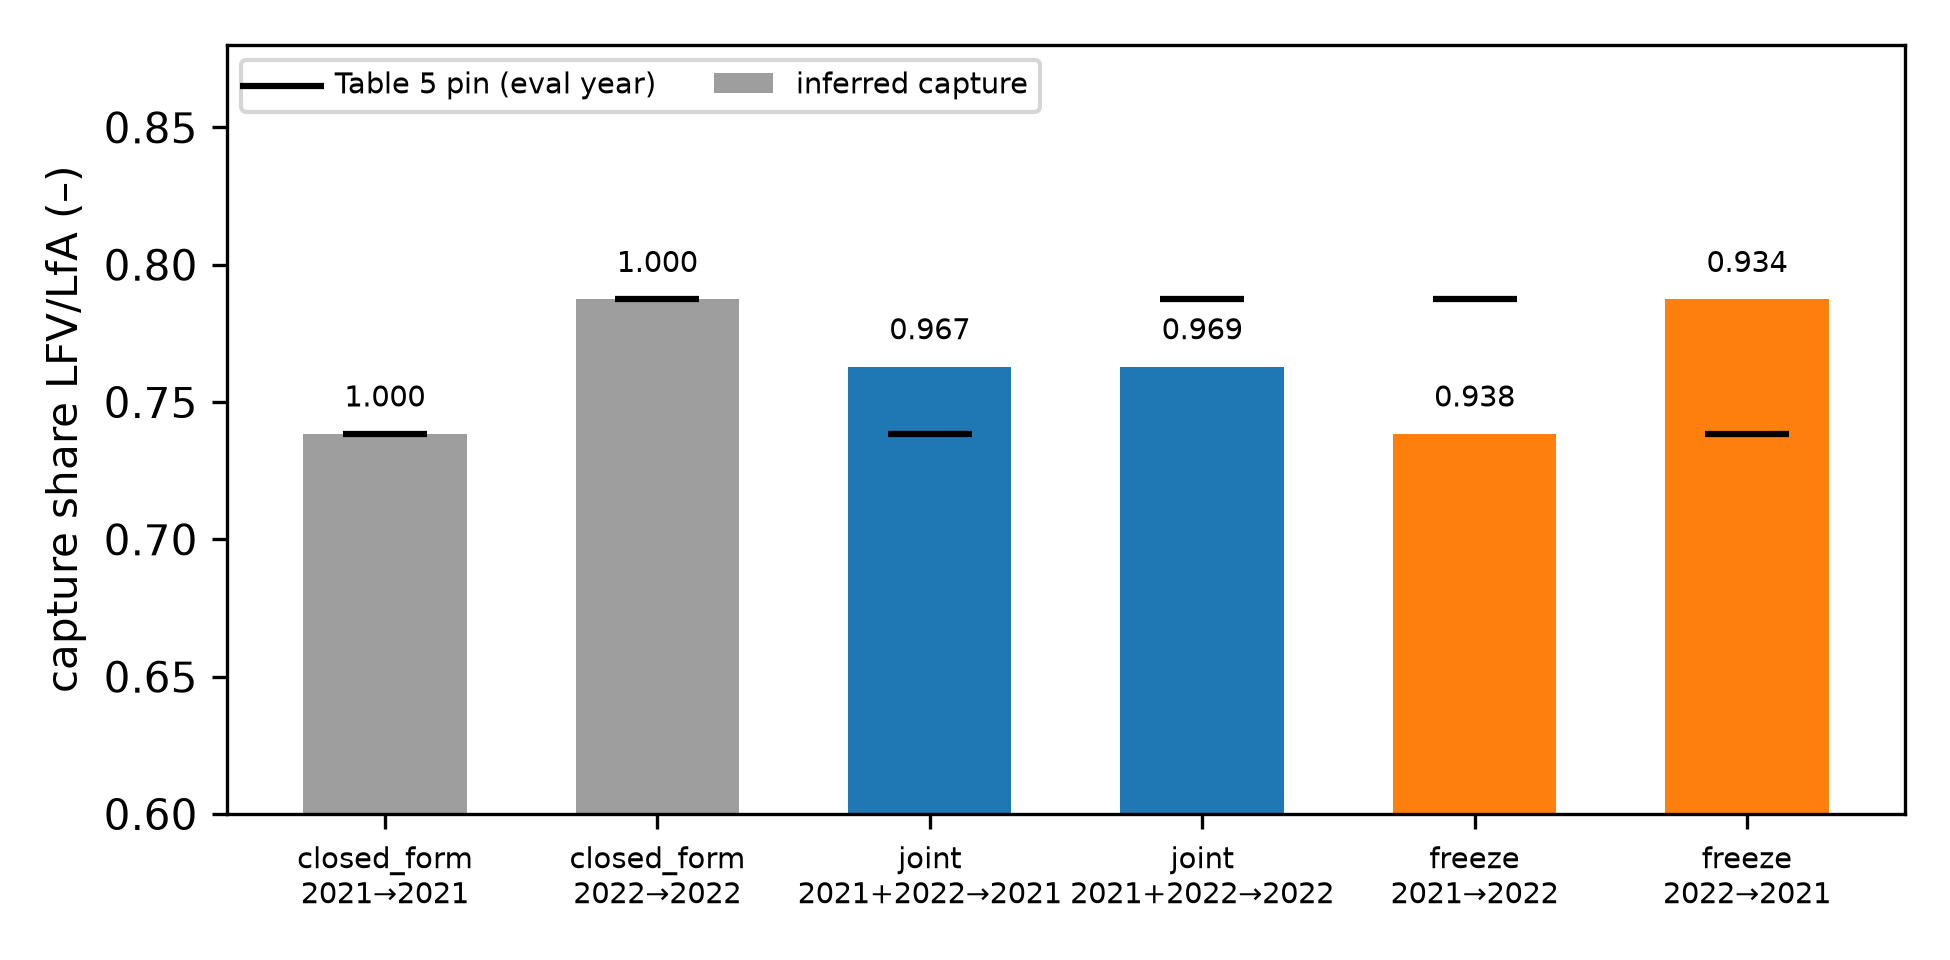
\includegraphics[width=0.85\linewidth]{fig2_capture_protocols.png}
\caption{Inferred district capture (bars) and evaluation-year Table~5 pin (marks); numbers are fidelities.}
\label{fig:capture}
\end{figure}

The closed form is exact by construction. The joint field sits between the two annual pins (mean fidelity 0.968)---the best attainable for any year-invariant field under this metric \citep{beven2006}. Neighbour exchange and on-plot storage each take 0.119 of positive leftover under the joint field.

\subsection{Farmer baselines}

\begin{table}[htbp]
\centering
\footnotesize
\caption{Season-total fidelity of registered farmer policies (irrigation is a decision).}
\label{tab:farmers}
\begin{tabular}{llcccc}
\toprule
Policy & Year & Fidelity & Irrigation & Drainage & Loss \\
\midrule
rainfed & 2021 & 0.232 & 0.000 & 0.463 & 1.013 \\
flooded & 2021 & 0.311 & 0.406 & 0.216 & 0.886 \\
persist & 2021 & 0.232 & 0.000 & 0.463 & 1.013 \\
et\_follower & 2021 & 0.721 & 0.610 & 0.832 & 0.360 \\
satellite & 2021 & 0.799 & 0.791 & 0.808 & 0.357 \\
et\_match (oracle) & 2021 & 0.990 & 1.000 & 0.980 & 0.007 \\
rainfed & 2022 & 0.086 & 0.000 & 0.171 & 1.141 \\
flooded & 2022 & 0.619 & 0.468 & 0.771 & 0.321 \\
persist & 2022 & 0.086 & 0.000 & 0.171 & 1.141 \\
et\_follower & 2022 & 0.601 & 0.587 & 0.616 & 0.290 \\
satellite & 2022 & 0.206 & 0.001 & 0.411 & 0.991 \\
et\_match (oracle) & 2022 & 0.966 & 1.000 & 0.932 & 0.005 \\
\bottomrule
\end{tabular}
\end{table}

\begin{figure}[htbp]
\centering
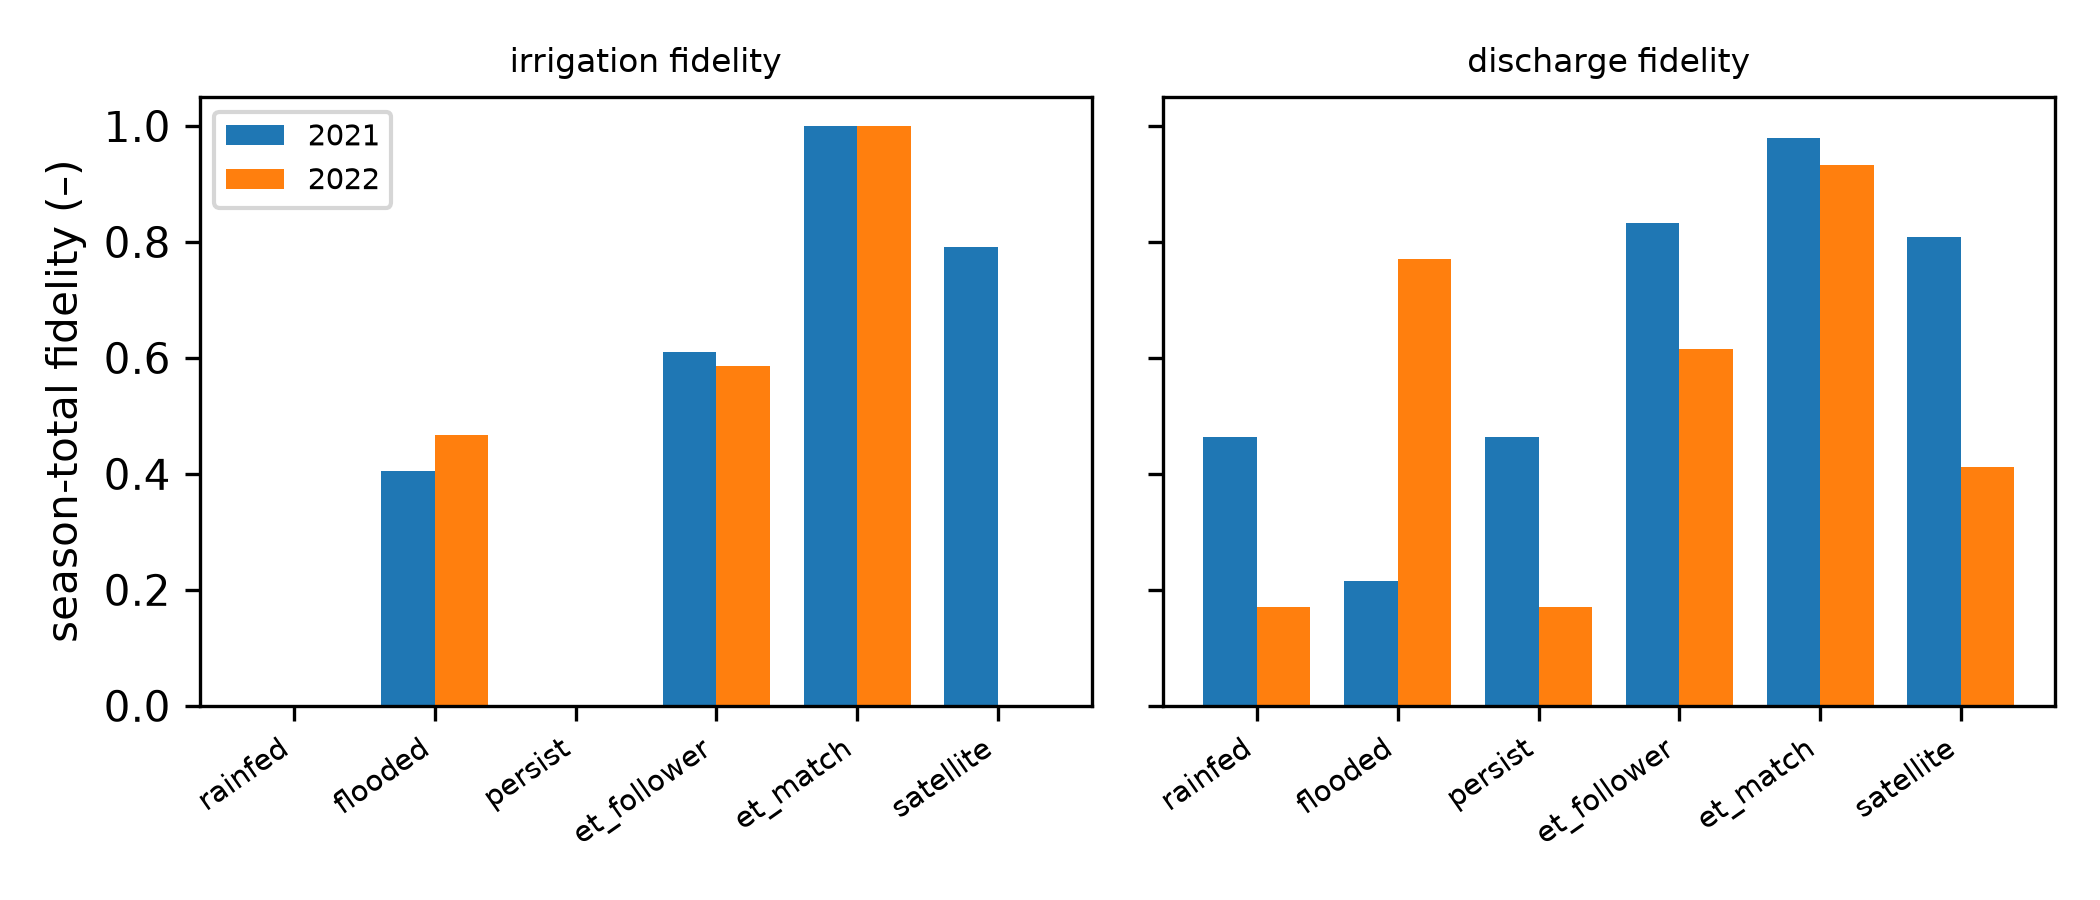
\includegraphics[width=0.85\linewidth]{fig3_farmer_track.png}
\caption{Irrigation and drainage season-total fidelity in wet (2021) and dry (2022) seasons.}
\label{fig:farmers}
\end{figure}

Three findings matter for benchmark users. First, \texttt{et\_match} reaches irrigation fidelity 1.000 because it redistributes observed totals; competitors must be compared on drainage and daily loss. Second, the satellite-driven rule is best non-oracle in 2021 (0.799) but collapses in dry 2022 (0.206)---year instability that a single-season evaluation would miss \citep{gauch2021}. Third, \texttt{persist} is identical to \texttt{rainfed} from a zero start.

\subsection{Gymnasium rollouts and observation masking}

\begin{table}[htbp]
\centering
\footnotesize
\caption{Full-season rollouts through \texttt{gymnasium.make}.}
\label{tab:gym}
\begin{tabular}{lllcccc}
\toprule
Env & Policy & Year & Reward & Drain.\ fid. & ET fid. & Steps\,s$^{-1}$ \\
\midrule
v0 & zero & 2021 & 0.696 & 0.764 & 0.911 & 6.4 \\
v0 & random & 2021 & 0.512 & 0.000 & 0.834 & 6.2 \\
v0 & spill 60 & 2021 & 0.696 & 0.764 & 0.911 & 5.8 \\
v0 & spill 20 & 2021 & 0.661 & 0.382 & 0.910 & 6.5 \\
v0 & et\_follower & 2021 & 0.670 & 0.535 & 0.909 & 6.2 \\
v0 & zero & 2022 & 0.657 & 0.851 & 0.825 & 7.6 \\
v0 & random & 2022 & 0.522 & 0.178 & 0.697 & 6.9 \\
v0 & spill 60 & 2022 & 0.657 & 0.851 & 0.825 & 6.6 \\
v0 & spill 20 & 2022 & 0.639 & 0.816 & 0.823 & 6.1 \\
v0 & et\_follower & 2022 & 0.629 & 0.880 & 0.810 & 6.5 \\
Open & et\_follower & 2021 & 0.701 & 0.832 & 0.942 & 27.7 \\
Open & et\_follower & 2022 & 0.681 & 0.616 & 0.916 & 27.1 \\
\bottomrule
\end{tabular}
\end{table}

In the known-irrigation environment, zero discharge obtains the highest mean reward in both years: with irrigation pinned, outlet overflow already produces drainage close to the observations, so active discharge must beat doing nothing \citep{kelly2024}. Open-environment \texttt{et\_follower} scores match the native loop exactly, confirming that the Gymnasium wrapper adds no hidden transformation.

\begin{table}[htbp]
\centering
\footnotesize
\caption{Observation-masking ablation for \texttt{et\_follower}.}
\label{tab:mask}
\begin{tabular}{llcccc}
\toprule
Env & Year & Dim. & Reward & Irr.\ fid. & Drain.\ fid. \\
\midrule
v0, shown & 2021 & 50 & 0.6699 & (pinned) & 0.5345 \\
v0, hidden & 2021 & 47 & 0.6699 & (pinned) & 0.5345 \\
v0, shown & 2022 & 50 & 0.6286 & (pinned) & 0.8795 \\
v0, hidden & 2022 & 47 & 0.6286 & (pinned) & 0.8795 \\
Open, shown & 2021 & 50 & 0.7013 & 0.6095 & 0.8321 \\
Open, hidden & 2021 & 47 & 0.7013 & 0.6091 & 0.8322 \\
Open, shown & 2022 & 50 & 0.6811 & 0.5869 & 0.6160 \\
Open, hidden & 2022 & 47 & 0.6807 & 0.5852 & 0.6147 \\
\bottomrule
\end{tabular}
\end{table}

With irrigation pinned, hiding the satellite pack cannot change this farmer's outcome---a negative control that masking does not leak into the physics.

\subsection{Hop-law holdout}

\begin{table}[htbp]
\centering
\footnotesize
\caption{Hop laws and leftover-fate regressions fitted on 2021, frozen for 2022 (RMSE, mm\,d$^{-1}$).}
\label{tab:hops}
\begin{tabular}{llcccc}
\toprule
Equation & Form & Scope & Params & 2021 RMSE & 2022 RMSE \\
\midrule
Neighbour hop & head\_equalise & general & 0 & 0.0000 & 0.0153 \\
Neighbour hop & linear & general & 14 & 0.0060 & 0.0016 \\
Neighbour hop & nonlinear & general & 26 & 0.0057 & 0.0050 \\
Neighbour hop & linear & per paddy & 68{,}950 & 0.0012 & 0.0197 \\
Recapture & affine & general & 9 & 1.367 & 2.977 \\
Recapture & affine & per paddy & 44{,}325 & 0.0019 & 1.108 \\
\bottomrule
\end{tabular}
\end{table}

On the held-out 2022 target, the 14-parameter linear law has about a tenth of the physics operator's error. The per-paddy law fits 2021 best and generalises worst---a textbook overfit that the protocol exposes. All hop fluxes are small, and all targets are simulator outputs; none of these numbers is a field validation.

%% ------------------------------------------------------------------
\section{Discussion}
\label{sec:discussion}

\subsection{What the environment makes possible}

CyclicEnv turns the published Imbanuma water balance \citep{okura2025} into an executable object with three registered slots matching surface decisions, leftover partition and neighbour exchange. That split follows EMS evaluation norms \citep{jakeman2006,bennett2013} and simulation-based control practice \citep{giuliani2021}. Bund and toposequence studies \citep{janssen2009,tsubo2007} justify neighbour shares; efficiency debates \citep{perry2007,grafton2018} justify scoring capture rather than claimed savings. Gymnasium \citep{towers2024}, crop and basin gyms \citep{kelly2024,osika2026} and EMS open-water packages \citep{tomlinson2020,hamilton2024,raming2025} define the niche. Year holdouts \citep{gauch2021} and hybrid process--learning arguments \citep{reichstein2019,nearing2021} match the frozen-physics design.

\subsection{Lessons for benchmark design}

\begin{itemize}
\item \textbf{Oracle leakage.} Any policy that sees observed block totals scores near-perfectly on irrigation; \texttt{et\_match} is package-internal.
\item \textbf{Year instability.} The satellite farmer collapses from wet 2021 to dry 2022 \citep{gauch2021}.
\item \textbf{Strong null.} Zero discharge wins in \texttt{Cyclic-Imbanuma-v0}; active policies must beat that baseline \citep{kelly2024}.
\item \textbf{Capacity versus transfer.} Per-paddy hop laws overfit the holdout protocol.
\item \textbf{Equifinality bound.} A year-invariant capture field cannot exceed about 0.968 mean fidelity \citep{beven2006}.
\item \textbf{Fig.~8 versus $IR_{\mathrm{all}}$.} Cyclic hard-copy matches Fig.~8; $IR_{\mathrm{all}}$ includes NCB supply \citep{okura2025}.
\end{itemize}

\subsection{Limitations}

The environment covers one district and two seasons. Daily irrigation is digitised and drainage is a rescaled monthly shape. The hop teacher is a modelling assumption, not a measurement. East--west versus north--south neighbour shares are not identifiable. FAO-56 parameters are defaults. Throughput with pinned irrigation (about 6--7 steps\,s$^{-1}$) limits sample-hungry deep RL without vectorised copies.

\subsection{Future work}

Planned extensions include ingesting original logger series, vectorised and batched environments, additional seasons and districts, uncertainty ranges on the Table~4--5 pins, and a public leaderboard on a frozen package version for farmers, hop laws and multi-objective simulation optimisation \citep{giuliani2021,lemmen2024}.

%% ------------------------------------------------------------------
\section{Conclusions}
\label{sec:conclusions}

CyclicEnv is an open, tested Gymnasium package for a real cyclic-irrigation district. It separates known surface forcing from the unobserved partition of leftover water and exposes that partition through three registered slots with role-specific, maskable observations. Reference results establish what is achievable and what is not: about 0.97 recapture fidelity for a year-invariant field, strong year dependence of simple farmer rules, a zero-discharge null that active policies must beat, and clear overfitting of per-paddy hop laws. We offer the package, protocols and baselines as a common testbed for learning water fate---and for simulation-based optimisation---in reuse-based irrigation systems.

\section*{Data availability}
District parcel geometry, digitised Okura series and tables, Open-Meteo forcing and derived Sentinel-2 products are distributed with or retrieved by the package. Raw Sentinel-2 scenes are available from the Copernicus Data Space Ecosystem. Result tables and figures are regenerated by \texttt{scripts/ems\_experiments.py}. [Archived DOI pending.]

\section*{CRediT authorship contribution statement}
[To be completed.]

\section*{Declaration of competing interest}
The authors declare that they have no known competing financial interests or personal relationships that could have appeared to influence the work reported in this paper.

\section*{Acknowledgements}
The environment is built on the field campaign and water-balance analysis of Okura, Kamei and Kato \citep{okura2025}. [Funding to be added.]

%% ------------------------------------------------------------------
\begin{thebibliography}{99}

\bibitem[Allen et~al.(1998)]{allen1998}
Allen, R.G., Pereira, L.S., Raes, D., Smith, M., 1998. Crop Evapotranspiration --- Guidelines for Computing Crop Water Requirements. FAO Irrigation and Drainage Paper~56. FAO, Rome.

\bibitem[Barker et~al.(2022)]{barker2022}
Barker, M., Chue Hong, N.P., Katz, D.S., Lamprecht, A.-L., Martinez-Ortiz, C., Psomopoulos, F., et~al., 2022. Introducing the FAIR Principles for research software. Scientific Data 9, 622. \doi{10.1038/s41597-022-01710-x}

\bibitem[Bennett et~al.(2013)]{bennett2013}
Bennett, N.D., Croke, B.F.W., Guariso, G., Guillaume, J.H.A., Hamilton, S.H., Jakeman, A.J., et~al., 2013. Characterising performance of environmental models. Environmental Modelling \& Software 40, 1--20. \doi{10.1016/j.envsoft.2012.09.011}

\bibitem[Beven(2006)]{beven2006}
Beven, K., 2006. A manifesto for the equifinality thesis. Journal of Hydrology 320, 18--36. \doi{10.1016/j.jhydrol.2005.07.007}

\bibitem[Drusch et~al.(2012)]{drusch2012}
Drusch, M., Del Bello, U., Carlier, S., Colin, O., Fernandez, V., Gascon, F., et~al., 2012. Sentinel-2: ESA's optical high-resolution mission for GMES operational services. Remote Sensing of Environment 120, 25--36. \doi{10.1016/j.rse.2011.11.026}

\bibitem[Er-Raki et~al.(2007)]{erraki2007}
Er-Raki, S., Chehbouni, A., Guemouria, N., Duchemin, B., Ezzahar, J., Hadria, R., 2007. Combining FAO-56 model and ground-based remote sensing to estimate water consumptions of wheat crops in a semi-arid region. Agricultural Water Management 87, 41--54. \doi{10.1016/j.agwat.2006.02.004}

\bibitem[Gauch et~al.(2021)]{gauch2021}
Gauch, M., Mai, J., Lin, J., 2021. The proper care and feeding of CAMELS: How limited training data affects streamflow prediction. Environmental Modelling \& Software 135, 104926. \doi{10.1016/j.envsoft.2020.104926}

\bibitem[Gautron et~al.(2022)]{gautron2022}
Gautron, R., Padr\'on, E.J., Preux, P., Bigot, J., Maillard, O.-A., Emukpere, D., 2022. gym-DSSAT: a crop model turned into a reinforcement learning environment. arXiv:2207.03270.

\bibitem[Giuliani et~al.(2021)]{giuliani2021}
Giuliani, M., Lamontagne, J.R., Reed, P.M., Castelletti, A., 2021. A state-of-the-art review of optimal reservoir control for managing conflicting demands in a changing world. Water Resources Research 57, e2021WR029927. \doi{10.1029/2021WR029927}

\bibitem[Grafton et~al.(2018)]{grafton2018}
Grafton, R.Q., Williams, J., Perry, C.J., Molle, F., Ringler, C., Steduto, P., et~al., 2018. The paradox of irrigation efficiency. Science 361, 748--750. \doi{10.1126/science.aat9314}

\bibitem[Hama et~al.(2010)]{hama2010}
Hama, T., Nakamura, K., Kawashima, S., 2010. Effectiveness of cyclic irrigation in reducing suspended solids load from a paddy-field district. Agricultural Water Management 97, 483--489. \doi{10.1016/j.agwat.2009.11.009}

\bibitem[Hamilton et~al.(2024)]{hamilton2024}
Hamilton, A.L., Amestoy, T.J., Reed, P.M., 2024. Pywr-DRB: An open-source Python model for water availability and drought risk assessment in the Delaware River Basin. Environmental Modelling \& Software 181, 106185. \doi{10.1016/j.envsoft.2024.106185}

\bibitem[Hutton et~al.(2016)]{hutton2016}
Hutton, C., Wagener, T., Freer, J., Han, D., Duffy, C., Arheimer, B., 2016. Most computational hydrology is not reproducible, so is it really science? Water Resources Research 52, 7548--7555. \doi{10.1002/2016WR019285}

\bibitem[Jakeman et~al.(2006)]{jakeman2006}
Jakeman, A.J., Letcher, R.A., Norton, J.P., 2006. Ten iterative steps in development and evaluation of environmental models. Environmental Modelling \& Software 21, 602--614. \doi{10.1016/j.envsoft.2006.01.004}

\bibitem[Janssen et~al.(2009)]{janssen2009}
Janssen, M., Lennartz, B., W\"ohling, T., 2009. Water losses through paddy bunds: Methods, experimental data, and simulation studies. Journal of Hydrology 369, 142--153. \doi{10.1016/j.jhydrol.2009.02.038}

\bibitem[Kaelbling et~al.(1998)]{kaelbling1998}
Kaelbling, L.P., Littman, M.L., Cassandra, A.R., 1998. Planning and acting in partially observable stochastic domains. Artificial Intelligence 101, 99--134. \doi{10.1016/S0004-3702(98)00023-X}

\bibitem[Kelly and Foster(2021)]{kelly2021}
Kelly, T.D., Foster, T., 2021. AquaCrop-OSPy: Bridging the gap between research and practice in crop-water modeling. Agricultural Water Management 254, 106976. \doi{10.1016/j.agwat.2021.106976}

\bibitem[Kelly et~al.(2024)]{kelly2024}
Kelly, T.D., Foster, T., Schultz, D.M., 2024. Assessing the value of deep reinforcement learning for irrigation scheduling. Smart Agricultural Technology 7, 100403. \doi{10.1016/j.atech.2024.100403}

\bibitem[Lemmen et~al.(2024)]{lemmen2024}
Lemmen, C., Sommer, P.S., et~al., 2024. Good modelling software practices. Ecological Modelling 498, 110890. \doi{10.1016/j.ecolmodel.2024.110890}

\bibitem[Nearing et~al.(2021)]{nearing2021}
Nearing, G.S., Kratzert, F., Sampson, A.K., Pelissier, C.S., Klotz, D., Frame, J.M., et~al., 2021. What role does hydrological science play in the age of machine learning? Water Resources Research 57, e2020WR028091. \doi{10.1029/2020WR028091}

\bibitem[Okura et~al.(2025)]{okura2025}
Okura, F., Kamei, A., Kato, T., 2025. Water balance analysis of hydrological processes in cyclic irrigation: A case study of the Imbanuma irrigation area in Chiba, Japan. Journal of Hydrology: Regional Studies 57, 102111. \doi{10.1016/j.ejrh.2024.102111}

\bibitem[Osika et~al.(2026)]{osika2026}
Osika, Z., R\u{a}dulescu, R., Zatarain Salazar, J., Oliehoek, F.A., Murukannaiah, P.K., 2026. MORL4Water: A modular multi-objective reinforcement learning toolkit for water resource management. \doi{10.65109/vsuw5215}

\bibitem[Overweg et~al.(2021)]{overweg2021}
Overweg, H., Berghuijs, H.N.C., Athanasiadis, I.N., 2021. CropGym: a reinforcement learning environment for crop management. arXiv:2104.04326.

\bibitem[Perry(2007)]{perry2007}
Perry, C., 2007. Efficient irrigation; inefficient communication; flawed recommendations. Irrigation and Drainage 56, 367--378. \doi{10.1002/ird.323}

\bibitem[Raffin et~al.(2021)]{raffin2021}
Raffin, A., Hill, A., Gleave, A., Kanervisto, A., Ernestus, M., Dormann, N., 2021. Stable-Baselines3: Reliable reinforcement learning implementations. Journal of Machine Learning Research 22~(268), 1--8.

\bibitem[Raming et~al.(2025)]{raming2025}
Raming, L.W., Vivoni, E.R., Cederstrom, C.J., Hossain, M.A., Becerra, J.A., 2025. pytRIBS: An open, modular, and reproducible python-based framework for distributed hydrologic modeling. Environmental Modelling \& Software 188, 106432. \doi{10.1016/j.envsoft.2025.106432}

\bibitem[Reichstein et~al.(2019)]{reichstein2019}
Reichstein, M., Camps-Valls, G., Stevens, B., Jung, M., Denzler, J., Carvalhais, N., Prabhat, 2019. Deep learning and process understanding for data-driven Earth system science. Nature 566, 195--204. \doi{10.1038/s41586-019-0912-1}

\bibitem[Sutton and Barto(2018)]{sutton2018}
Sutton, R.S., Barto, A.G., 2018. Reinforcement Learning: An Introduction, 2nd~ed. MIT Press, Cambridge, MA.

\bibitem[Takeda et~al.(1997)]{takeda1997}
Takeda, I., Fukushima, A., Tanaka, R., 1997. Non-point pollutant reduction in a paddy-field watershed using a circular irrigation system. Water Research 31, 2685--2692. \doi{10.1016/S0043-1354(97)00117-6}

\bibitem[Tomlinson et~al.(2020)]{tomlinson2020}
Tomlinson, J.E., Arnott, J.H., Harou, J.J., 2020. A water resource simulator in Python. Environmental Modelling \& Software 126, 104635. \doi{10.1016/j.envsoft.2020.104635}

\bibitem[Towers et~al.(2024)]{towers2024}
Towers, M., Kwiatkowski, A., Terry, J., Balis, J.U., De Cola, G., Deleu, T., et~al., 2024. Gymnasium: A standard interface for reinforcement learning environments. arXiv:2407.17032.

\bibitem[Tsubo et~al.(2007)]{tsubo2007}
Tsubo, M., Fukai, S., Tuong, T.P., Ouk, M., 2007. A water balance model for rainfed lowland rice fields emphasising lateral water movement within a toposequence. Ecological Modelling 204, 503--515. \doi{10.1016/j.ecolmodel.2007.02.001}

\bibitem[Tsuchiya et~al.(2018)]{tsuchiya2018}
Tsuchiya, R., Kato, T., Jeong, J., Arnold, J.G., 2018. Development of SWAT-Paddy for simulating lowland paddy fields. Sustainability 10, 3246. \doi{10.3390/su10093246}

\bibitem[Walker and Rushton(1986)]{walker1986}
Walker, S.H., Rushton, K.R., 1986. Water losses through the bunds of irrigated rice fields interpreted through an analogue model. Agricultural Water Management 11, 59--73. \doi{10.1016/0378-3774(86)90036-3}

\bibitem[Zippenfenig(2023)]{zippenfenig2023}
Zippenfenig, P., 2023. Open-Meteo.com Weather API. Zenodo. \doi{10.5281/zenodo.7970649}

\end{thebibliography}

%% ------------------------------------------------------------------
\appendix

\section{Reproducing the results}
\label{app:repro}

\begin{lstlisting}[language=Bash]
pip install -e ".[ems]"
python -m unittest discover -s tests
python scripts/ems_experiments.py
\end{lstlisting}

\begin{table}[htbp]
\centering
\small
\caption{Script outputs mapped to article items.}
\begin{tabular}{ll}
\toprule
Output & Article item \\
\midrule
\texttt{ratios.csv}, \texttt{fig2\_*.png} & Table~\ref{tab:capture}, Fig.~\ref{fig:capture} \\
\texttt{farmers.csv}, \texttt{fig3\_*.png} & Table~\ref{tab:farmers}, Fig.~\ref{fig:farmers} \\
\texttt{gym\_rollouts.csv} & Tables~\ref{tab:gym}--\ref{tab:mask} \\
\texttt{equations.csv} & Table~\ref{tab:hops} \\
\texttt{observation\_roles.csv} & Table~\ref{tab:obs} \\
\bottomrule
\end{tabular}
\end{table}

\section{Registering a new hop law}
\label{app:register}

\begin{lstlisting}
import numpy as np
import cyclic

@cyclic.register_lateral("my_hops")
class MyHops(cyclic.LateralPolicy):
    def flux(self, stock, graph, area, physics,
             neighbour_et_mm=None, et_mm=None):
        after = np.asarray(stock, dtype=float).copy()
        # move leftover between graph neighbours
        return after, after - stock

report = cyclic.soil_flow_holdout(
    train_year=2021, eval_year=2022, equation="my_hops")
\end{lstlisting}

\end{document}
